\documentclass[../TV&MS.tex]{subfiles}

\begin{document}
\section{Условная вероятность. Независимость событий}

\qquadРассмотрим произвольное $B \in \Ev \colon \quad \Pro(B) > 0$.
\begin{Def}
\underline{Условной вероятностью} события $A \in \Ev$ при условии $B$ называется $\frac{\Pro(AB)}{\Pro(B)} =\colon \Pro(A|B) = \Pro_B(A)$
\end{Def}

Что это означает на пальцах? Условная вероятность $\Pro(A|B)$ --- это веротяность того, что произойдет событие $A$, если мы точно знаем, что произошло событие $B$.\\

\parbox[b][3 cm][t]{20mm}{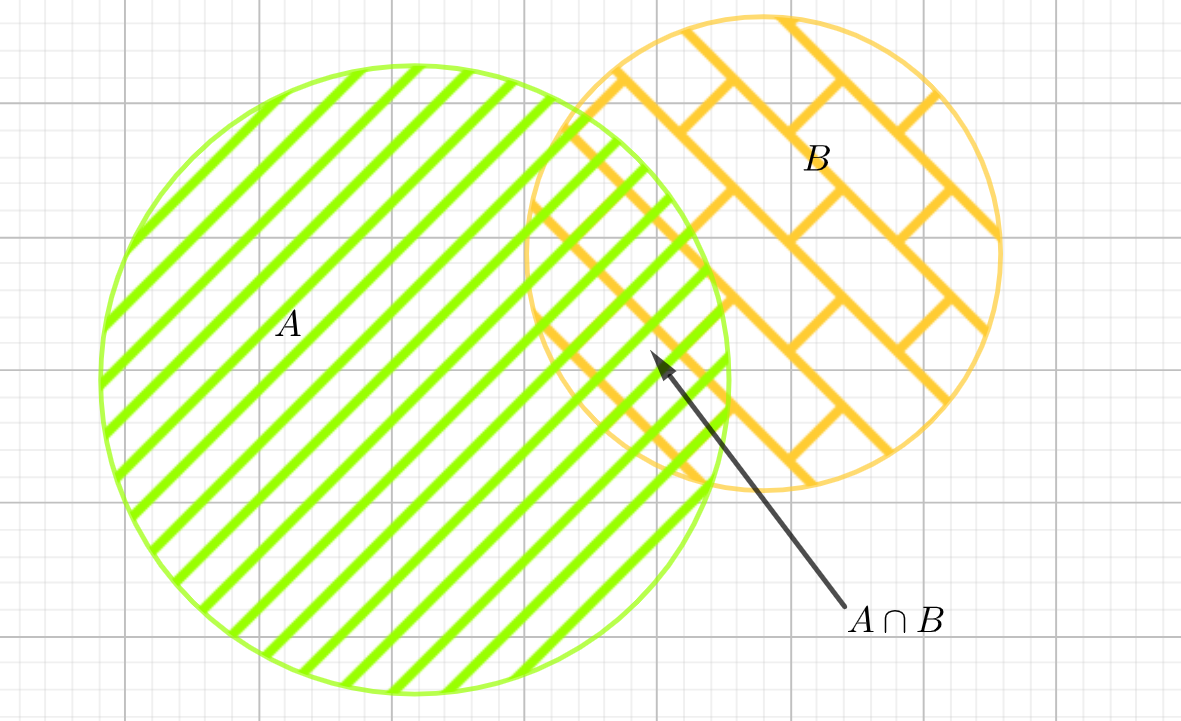
\includegraphics[height=30mm]{cond_prob}}
\hfill
\parbox[b][3 cm][t]{100mm}{
	Графически это означает, что, когда произошло событие $B$, мы оказались в круге $B$. Тогда формула  $\frac{\Pro(AB)}{\Pro(B)}$ есть просто вероятность попасть в $AB$.
}\\

Из определения следует так называемый <<Закон умножения вероятностей>>:
$$\Pro(A|B)\Pro(B)=\Pro(AB)$$

Легко проверяется, что $(B, \Ev_B, \Pro_B)$, где $\Ev_B = \Set{A \bigcap B}{A \in \Ev}$, так же является вероятностным пространством. \\
\begin{Wtf}
Зачем нужно требование $\Pro(B) > 0$, если можно в случае $\Pro(B) = 0$ доопределить условную вероятность нулем как вероятность при условии невозможного события?
При таком доопределении нарушится аксиома 3. вероятности $\Pro_B$, поскольку $\Pro_B(B)$ по доопределению будет равно $0$.
\end{Wtf}

\begin{Def}
События $A, B \in \Ev$ называются \underline{независимыми}, если $$\Pro(AB) = \Pro(A) \Pro(B)$$.
\end{Def}

Для независимых событий $$\Pro(A|B) = \frac{\Pro(A)\Pro(B)}{\Pro(B)} = \Pro(A)$$.\\
\begin{Ex}
Являются ли несовместные события ($AB = \varnothing$) независимыми? Нет, пусть  $A, B \in \Ev \colon \quad \Pro(A) > 0, \ \Pro(B) > 0$. Тогда $\Pro(AB) = \Pro(A)\Pro(B) = 0$, 
что является противоречием. По-простому, если произошло одно из несовместных событий, то второе уже не может произойти, и его условная веротяность равна 0, а не
вероятности самого события, что требуется для независимости.
\end{Ex}

Следующее определение обобщает понятие независимости на произвольное количество событий.
\begin{Def}
События $A_1, A_2, \dots, A_n$ называются \underline{независимыми в совокупности}, если 
$$\forall m = 2, \dots, n \quad \forall 1 \le j_1 < \ldots < j_m \le n \quad 
\Pro(\bigcap_{k=1}^{m}A_{j_k})=\prod_{k=1}^{m} \Pro(A_{j_k})$$
\end{Def}
\begin{Ex}
На примере тетраэдра Бернштейна можно убедиться в том, что попарной независимости событий недостаточно для независимости в совокупности. Рассмотри тетраэдр, у 
которого три стороны покрашены в красный, синий и зеленый, а четвертая содержит все три цвета. События \{выпадет красный\}=\{К\}, \{выпадет синий\}=\{С\}, \{выпадет зеленый\}=\{З\}
попарно независимы (например, вероятность события \{С\}$\bigcap$\{К\} равна веротяности выпадения четвертой грани, т. е. $\frac{1}{4}$, в то время как выпадения 
каждого цвета равна $\frac12$). Однако $\Pro$(\{С\}$\bigcap$ \{К\}$\bigcap$ \{З\}) = $\frac14 \not= (\frac12)^3$.
\end{Ex}
\newpage


\end{document}
